\documentclass{article}
\usepackage{amsmath}
\usepackage{amssymb}
\usepackage{graphicx}
\usepackage{float}
\usepackage{enumitem}
\usepackage{forest}

\begin{document}

\title{Homework 4}
\author{Manyara Bonface Baraka - mbaraka}
\date{\today}
\maketitle

\section*{Problem 1: Bayesian Learning}
\textit{Bayesian Learning calculates the probability of  each hypothesis given the data, and makes predictions by weighing all hypothesis by their probabilities}

- Will asssumed eaqual prior start for each hypothesis \(P(h_i) = \frac{1}{6}\) for all i
\subsubsection*{Observations}
\textbf{Plots}
\begin{figure}[H]
    \centering
    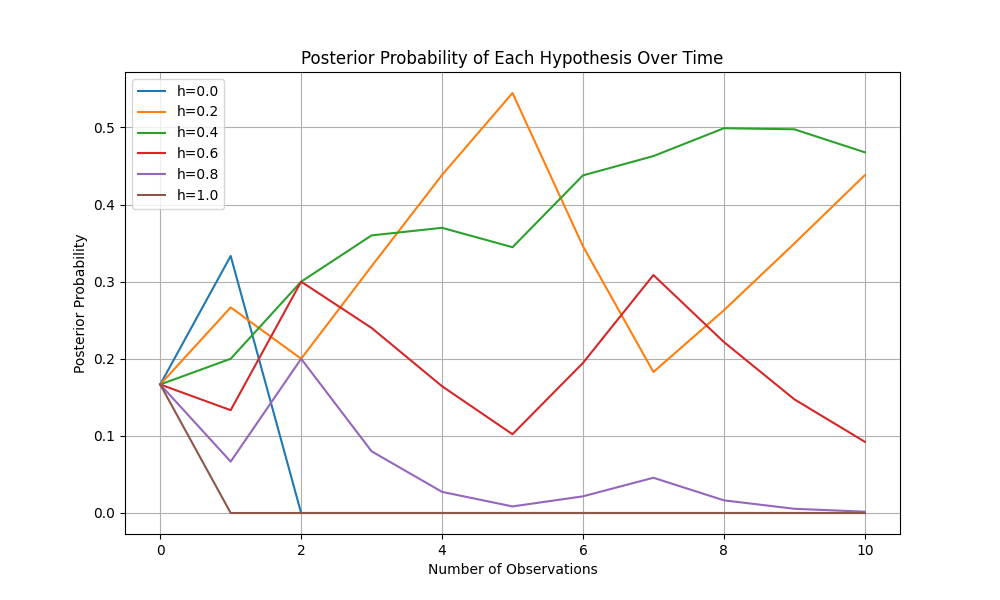
\includegraphics[width=0.8\textwidth]{../Problem1/num_of_observation.png}
    % \caption{Number of Observations}
    \label{fig:num_of_observation}
\end{figure}

\begin{figure}[H]
    \centering
    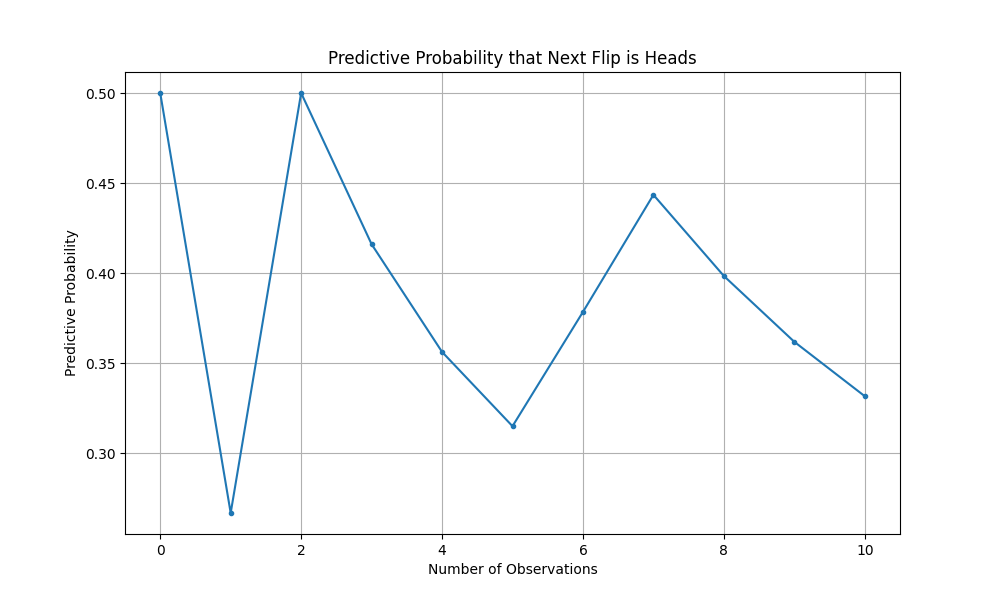
\includegraphics[width=0.8\textwidth]{../Problem1/predictive_of_next_head.png}
    % \caption{Number of Observations}
    \label{fig:num_of_observation}
\end{figure}

\textbf{Most likely hypothesis after all observations: h=0.4}

\subsubsection*{Insights}

\textbf{The first plot: Posterior Probability plot}: the plot shows the evolution of the posterior probabilities over time for each hypothesis.
At the start all hypthesis have the same prior however as the observation came in the posterior changes am having the likely of h=0.4.\\
\textbf{The second plot: Predictive Probabilit plot}: the second plot depicts teh predictive probability that the next flip will be heads, calculate after each observation.
The model flactuates at first but it tends to stabilize around 0.4. The highest posterior probabily influences the dominance of the hypthesis on predictions. The predictive 
probability tends to be stable aroung 0.4 since the posterior of h3 becaomes quite large. 


\clearpage

\section*{Problem 2: Maximum a Posteriori (MAP) Estimation}
\begin{figure}[H]
    \centering
    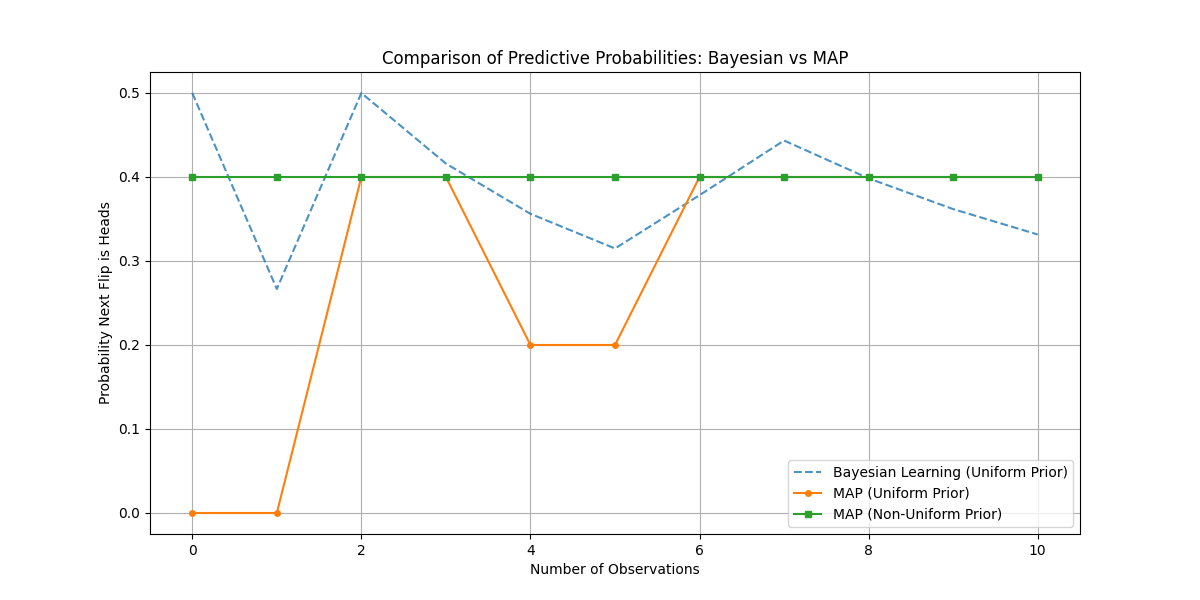
\includegraphics[width=0.8\textwidth]{../Problem2/Figure_1.png}
    % \caption{Number of Observations}
    \label{fig:num_of_observation}
\end{figure}

\subsubsection*{Observation and Insights}
\textbf{MAP vs Bayesian}

- Smoothness: Bayesian with the blue dotted it smoothly converge  to the true bias by averagin all hypthesis however, the MAP prediction jumps discretely as the most probable hypothesis changes.

- Prior sensistivity: With the uniform prior MAP predictions astarts at 0 due to limitation in tie-breaking but it adjusts faster as the data comes in. While with non-uniform
prior is biased  MAP initially predicts 0.4 and its constant for that. \\

Generally the MAP is computational efficinte however its prone to abrupt changes and prior bias, especially with limited data. It trades off accuracy for simplicity while Bayesian provides a robust predictions
by combining uncertinity but requires more computation.


\clearpage

\section*{Problem 3: Maximum Likelihood (ML) Estimation}
\begin{figure}[H]
    \centering
    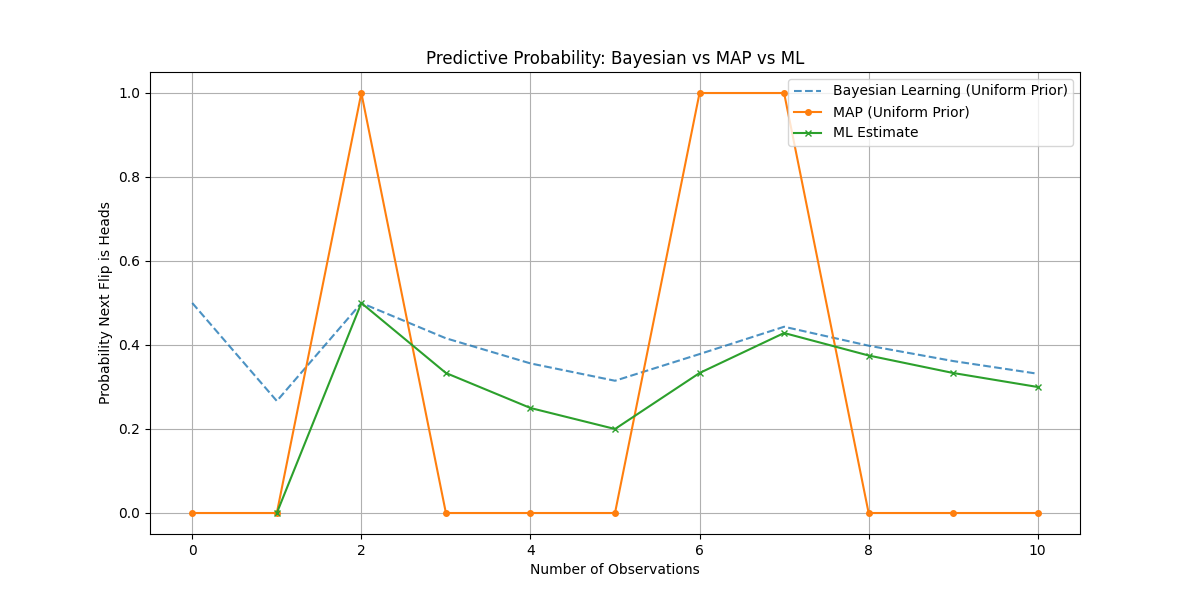
\includegraphics[width=0.8\textwidth]{../Problem3/Comparizon_ML_MAP_Bayesian.png}
    % \caption{Number of Observations}
    \label{fig:num_of_observation}
\end{figure}
\begin{itemize}
    \item Is the estimate equal to the estimates we found as a result of Bayesian Learning and MAP estimation? What is the major difference?
    \item Which is likely to be more accurate: the estimate found with ML estimation or the estimate found using the other methods?
    \item In what case (specifically, for what prior distribution) does MAP estimation reduce to the ML estimate? Feel free to consult Section 20.2 Learning with Complete Data in Russel \& Norvig.
    \item Provide a brief discussion comparing Bayesian Learning, MAP, and ML estimation. What are the pros and cons of each?
\end{itemize}


\end{document}